\documentclass[12pt,letterpaper]{article}
\usepackage{fullpage}
\usepackage[top=2cm, bottom=4.5cm, left=2.5cm, right=2.5cm]{geometry}
\usepackage{amsmath,amsthm,amsfonts,amssymb,amscd}
\usepackage{lastpage}
\usepackage{enumerate}
\usepackage{fancyhdr}
\usepackage{mathrsfs}
\usepackage{xcolor}
\usepackage{graphicx}
\usepackage{listings}
\usepackage{hyperref}
\usepackage{float}

\hypersetup{%
  colorlinks=true,
  linkcolor=blue,
  linkbordercolor={0 0 1}
}
 
\renewcommand\lstlistingname{Algorithm}
\renewcommand\lstlistlistingname{Algorithms}
\def\lstlistingautorefname{Alg.}

\lstdefinestyle{Python}{
    language        = Python,
    frame           = lines, 
    basicstyle      = \footnotesize,
    keywordstyle    = \color{blue},
    stringstyle     = \color{green},
    commentstyle    = \color{red}\ttfamily
}

\setlength{\parindent}{0.0in}
\setlength{\parskip}{0.05in}

% Edit these as appropriate
\newcommand\course{He-6 CRES Project}
\newcommand\hwnumber{CRES Kassiopeia Results}                  % <-- homework number
\newcommand\NetIDa{Alexander Allen}           % <-- NetID of person #1

\pagestyle{fancyplain}
\headheight 35pt
\lhead{\NetIDa}
\chead{\textbf{\Large \hwnumber}}
\rhead{\course \\ \today}
\lfoot{}
\cfoot{}
\rfoot{\small\thepage}
\headsep 1.5em

\begin{document}


\section{Introduction}

We present results for simulations using the Kassiopeia software developed for the Katrin experiment. Source code for the Kassiopeia project can be found \href{https://github.com/KATRIN-Experiment/Kassiopeia}{here}. 

These simulations establish a cylindrical experimentation space with the z-axis defined along the length of the cylinder. The cylinder is $10~$cm in length and has a radius of $1~$cm representing a wave guide.

At the center of the geometry there is a particle generator which generates electrons with kinetic energy of $511~$keV and an isotropic velocity distribution into a $2\pi$ solid angle in the positive z direction .

The purpose of this experiment is to establish the basic requirements for Kassiopeia to begin the construction of the complete CRES geometry and to validate that the simulations are returning results we expect and to evaluate their precision.

We first analyze the cyclotron motion of these generated particles under the application of a $1~$T magnetic field along the z-axis. Here we verify that conservation of energy is maintained, verify that the larmor radius is what we expect, and determine that the precision of the simulation is well within our tolerances by predicting the final location using the initial conditions and comparing it to the simulation results. 

Next, we analyze the same cyclotron motion with the addition of an E-field that creates electron drift. We calculate the location we expect to find the center of rotation of the electrons and then compare that to the center that is determined from the simulation. We then compute the theoretical drift velocity, adjust our predictions and calculate a second set of errors. We plot both of these errors over time and find that the predictions without accounting for drift have unbounded error while the predictions using the theoretical drift velocity have low and well bounded error values over time allowing us to confirm our simulation is behaving as expected. 

Next, we add a solenoidal magnetic field to the simulation to create an electron trap. We calculate the critical pitch angle for the electron to be trapped and we calculate the resulting trapping fraction of the population of electrons. We verify that larger pitch angles result in lower oscillation times and smaller magnetron motion. 

Finally, we add an electric field to the trapping geometry to model electron drift in the trap. We extract the time it takes trapped electrons to reach the edge of the geometry and plot that in a histogram. We determine that the emptying time for electrons in the trap generally resides between 5 and 50 nanoseconds and conclude that the electric field applied in the simulation is adequate for emptying the trap of charged particles in a reasonable time frame without the need to remove the magentic field. 

\section{Constant B-Field}

In the first experiment a constant magnetic field of magnitude 1 Tesla is applied globally along the positive z-axis. The active geometry is a cylinder of radius $0.01~$m and length $0.1~$m oriented along the z-axis and centered at the origin.

\subsection{Conservation of Energy}

Firstly we ensure that conservation of energy is held by plotting a histogram of change in kinetic energy from beginning to the end of the simulation for the population of electrons simulated. In an ideal scenario this is zero, thus this is a indicator of the error we are seeing in the built-in integrator. 

    \begin{figure}[H]
    \centering
    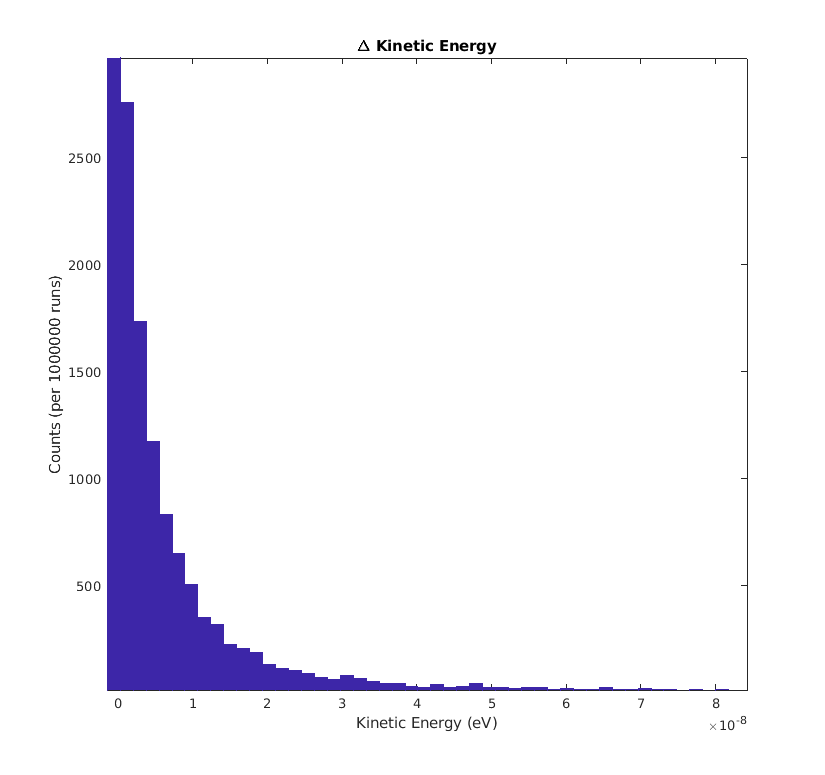
\includegraphics[width=0.7\linewidth]{ke.png}
    \caption{Change in kinetic energy}
    \end{figure}
    
We see here that the error generally lies less than $2\times10^{-8}~$eV which is a reasonable range given the $511\times10^{3}~$eV initial kinetic energy the electrons start with.

\subsection{Arrival Time Distribution}

Next we analyze the arrival times of the electrons to the end of the geometry. This is the time it takes for the electron to travel from its incident location to the end of the geometry 5cm from the generator. We use this metric to verify that the generator is isotropically distributing the initial momentum vector of the electrons as this assumption drives many other conclusions we can draw from this simulation. 

We use the arrival time to calculate a $v_z$ value by

\[ v_z = \frac{0.05}{t} \]

Given the kinetic energy of $511~$keV we calculate the total velocity of the electron to be $0.866c$ thus we can compute the ratio of the z-component velocity to the total velocity by

\[ \frac{v_z}{0.866c} \]

The isotopic distribution is defined as a uniform distribution over $cos(\theta)$ from zero to one.

\[ cos(\theta) = \frac{v_z}{0.866c} \]

Thus, we expect that the distribution of $\frac{v_z}{v}$ across the population of electrons be uniform.

    \begin{figure}[H]
    \centering
    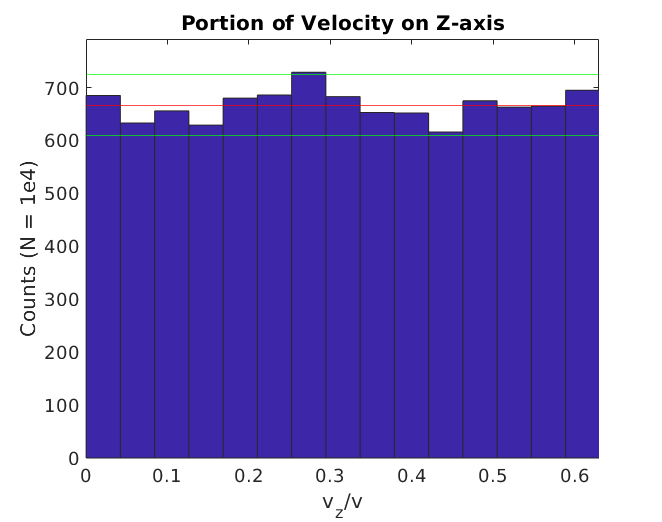
\includegraphics[width=0.7\linewidth]{arrival.png}
    \caption{Distribution of velocities parallel to the geometry}
    \end{figure}
    
We can see that this population sample shown here is uniform and thus the distribution of particle trajectories is likely isotropic. 

One feature of this histogram is that the deviation from the mean / uniform value increases as the velocity of the particle increases in the z direction. Due to the nature of the inverse function and floating point math in the simulation system, very small arrival times (which correspond to the higher velocities) are much more sensitive to small floating point errors and small errors originating from the numerical integrator (8th order Runge-Kutta) which is why we see the greater deviation. 

However, it can also be observed that these deviations are largely a factor of the binning of the histogram and that binning at larger intervals smooths out these deviations which supports the conclusion that the observed deviance is mostly random error rather than systematic. Additionally, the red and green lines on the chart represent the mean ($4247$) and 95\% point ($\pm 156$) of the count value and all counts fall within these bounds suggesting that our error is Gaussian.

\subsection{Larmor Radius}

Next, we analyze the Larmor radius of the particles as they travel down the geometry. We can predict the Larmor radius using the initial conditions of the particle by

\[ v_{t} = 0.866c\frac{p_x^2 + p_y^2}{p_x^2 + p_y^2 + p_z^2} \]
\[ \gamma = \frac{1}{\sqrt{1 - 0.866^2}} = 2 \]
\[ r = \frac{\gamma mv_t}{qB}  \]

Using this predicted radius we perform a 90 degree rotation of the x/y momentum vector to get a vector pointed towards the center of rotation and then apply a magnitude of the Larmor radius to get a vector which points from the initial position to the predicted rotational center.

For each step in the simulated particles trajectory we perform this same computation and calculate the predicted center of rotation. For each step we calculate the distance the center has drifted from the initial predicted center. 

We collect this error value for all steps, for all particles and present a histogram of these error values as well as a plot of the error over time for a sample particle to show how it varies over time.

    \begin{figure}[H]
    \centering
    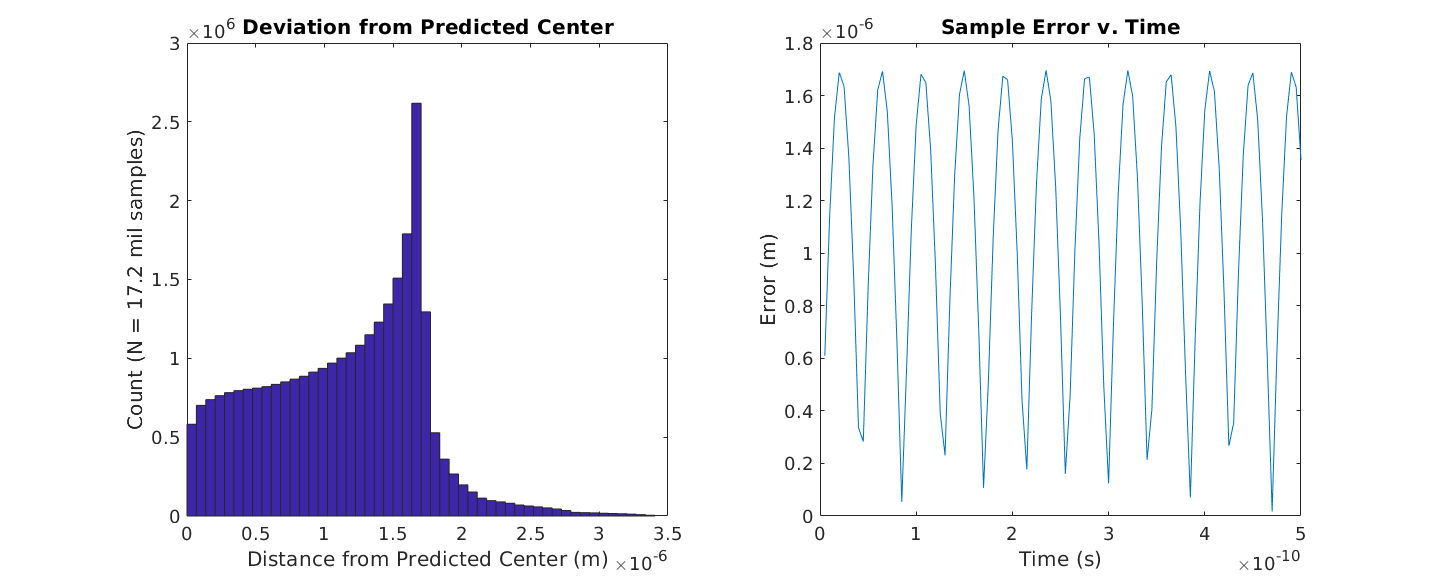
\includegraphics[width=\linewidth]{larmor.png}
    \caption{Larmor Radius Error}
    \end{figure}
    

Error values peak at $5~$nm and drop off significantly at $10~$nm which is an acceptably low value. This shows that the motion of the particle is indeed circular, tangent to its initial position, and matches the trajectory and velocity we expect given the simulation conditions. 

We also visualize the x/y projection of the trajectories of the particles as an additional layer of validation. The simulation boundary is super-imposed on this plot for visualization purposes. 

    \begin{figure}[H]
    \centering
    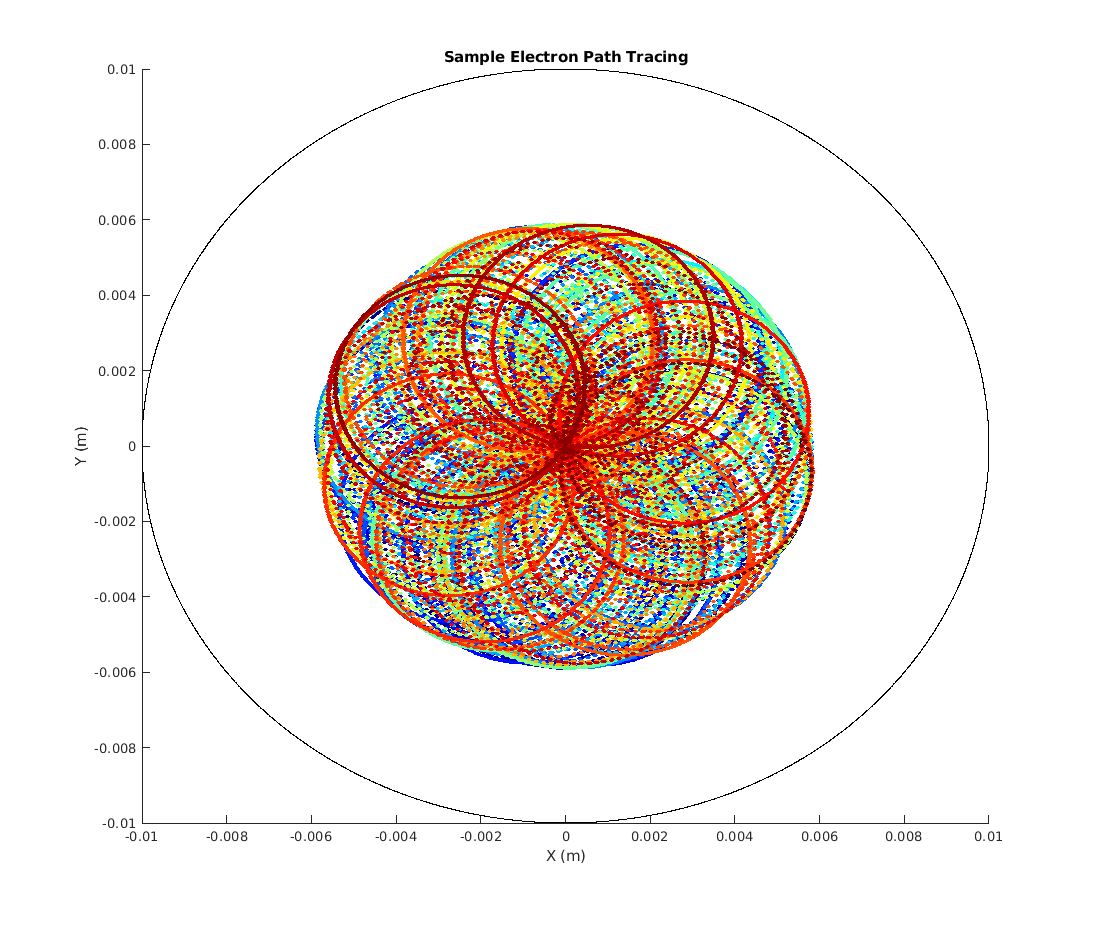
\includegraphics[width=0.9\linewidth]{track.png}
    \caption{Particle track visualization}
    \end{figure}

\subsection{Phase}
    
Finally, to evaluate the precision with which the simulation calculates particle paths, we use the initial conditions of the particle to predict the trajectory and final coordinates of the electron path in the x / y plane. To do this we once again evaluate the center of rotation using the computed Larmor radius and we also use the initial momentum to calculate the angular frequency around that center. We then use the momentum in the z direction to predict the arrival time of the particle and use that in conjunction with the angular frequency to predict the position of the particle when it terminates at the end of the geometry. 

We then look at the final position of the particle given by the simulation and compare it to the prediction. The value we compute for these positions is the displacement in radians around the center of the cyclotron motion from the initial condition to the final condition. 

We then visualize a histogram of errors across the particle population between the predicted phase and the phase reported by the simulation.

    \begin{figure}[H]
    \centering
    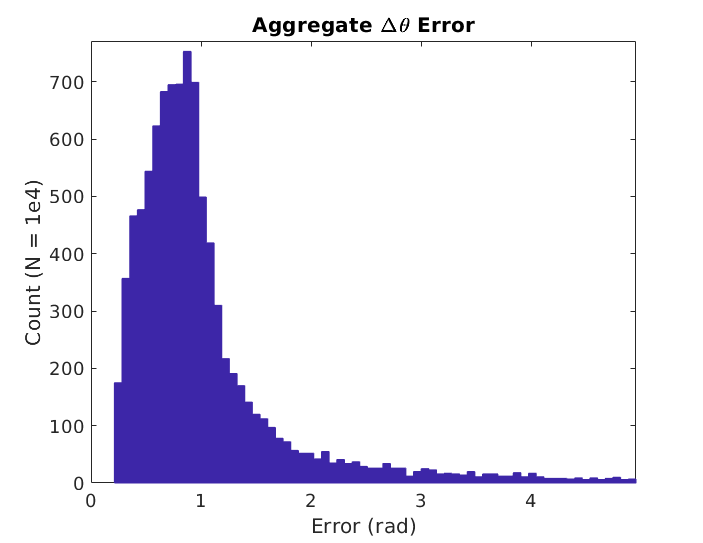
\includegraphics[width=0.7\linewidth]{phase.png}
    \caption{Phase error}
    \end{figure}
    
These errors are reported in radians and while there are a few outliers the error generally stays below $0.5~$rad and as such is acceptable to the precision necessary.

\section{ExB Field}

We then modify the simulation in Kassiopeia to include an electric field of magnitude $2e5$ in the negative y direction in the geometry. This will create a drift for the electrons.

    \begin{figure}[H]
    \centering
    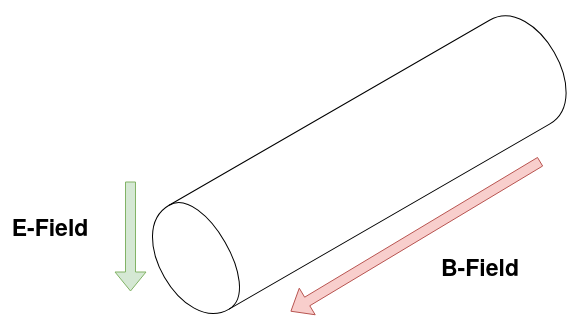
\includegraphics[width=0.8\linewidth]{CRES.png}
    \caption{Diagram of Simulation Geometry}
    \end{figure}

To validate this drift is occuring to the magnitude we expect we repeat the experiment in the previous section that tracks the center of the cyclotron motion of the particles. 

We expect to see error values between the initial center point and the final center point corresponding with the drift velocity created by the E-field. To verify this we apply a correction to the calculated center point based on the known magnitude of the ExB drift and expect that the errors will return to smaller values.

    \begin{figure}[H]
    \centering
    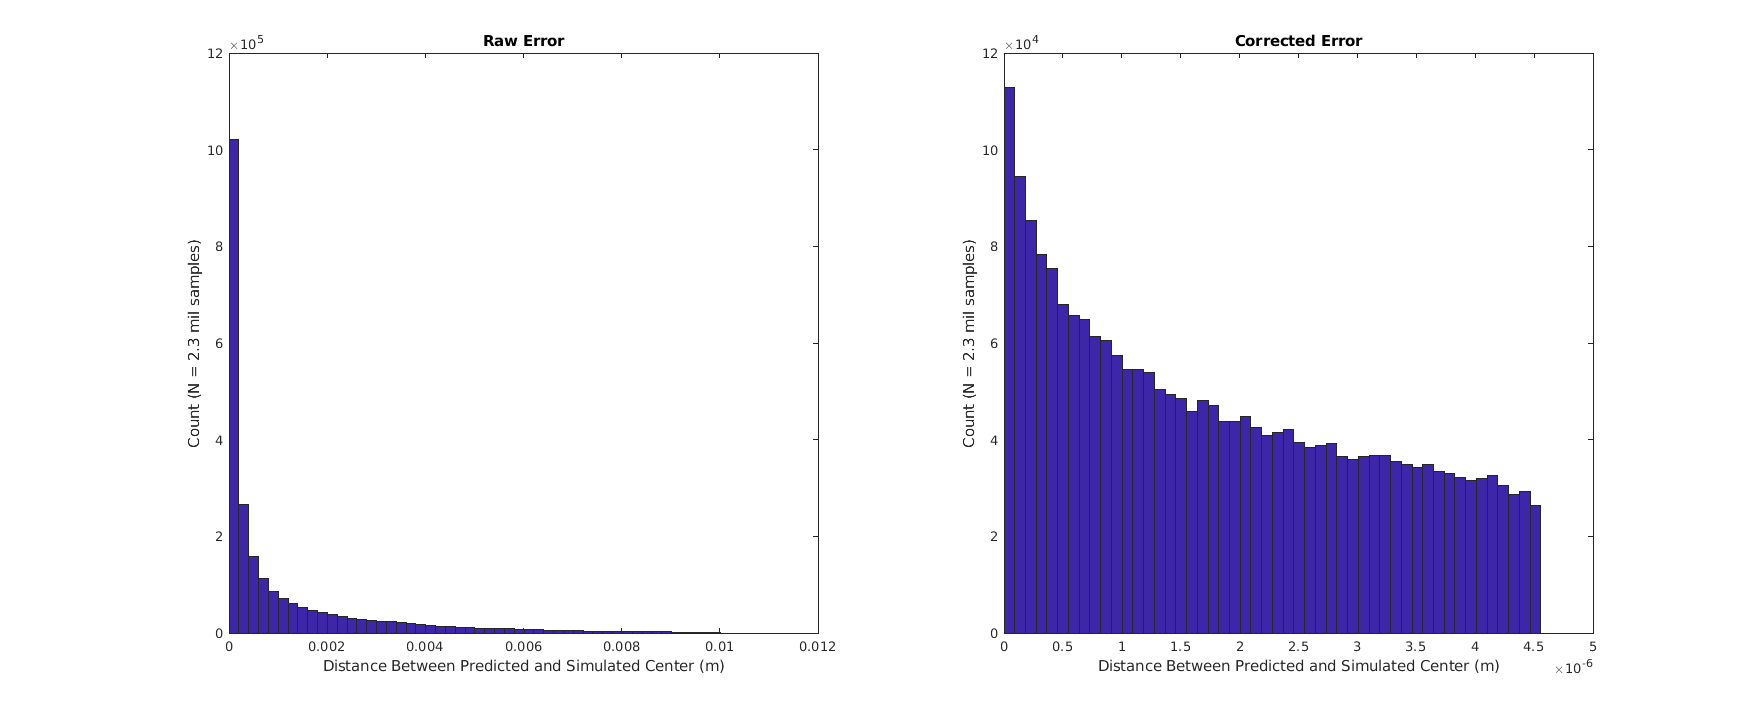
\includegraphics[width=0.9\linewidth]{drift.png}
    \caption{Drift Correction}
    \end{figure}

Here we observe the uncorrected error and corrected error differ by almost 2 orders of magnitude. The uncorrected error is also severely skewed to lower values which we expect as the particles slowly diverge from their expected centers over time. 

    \begin{figure}[H]
    \centering
    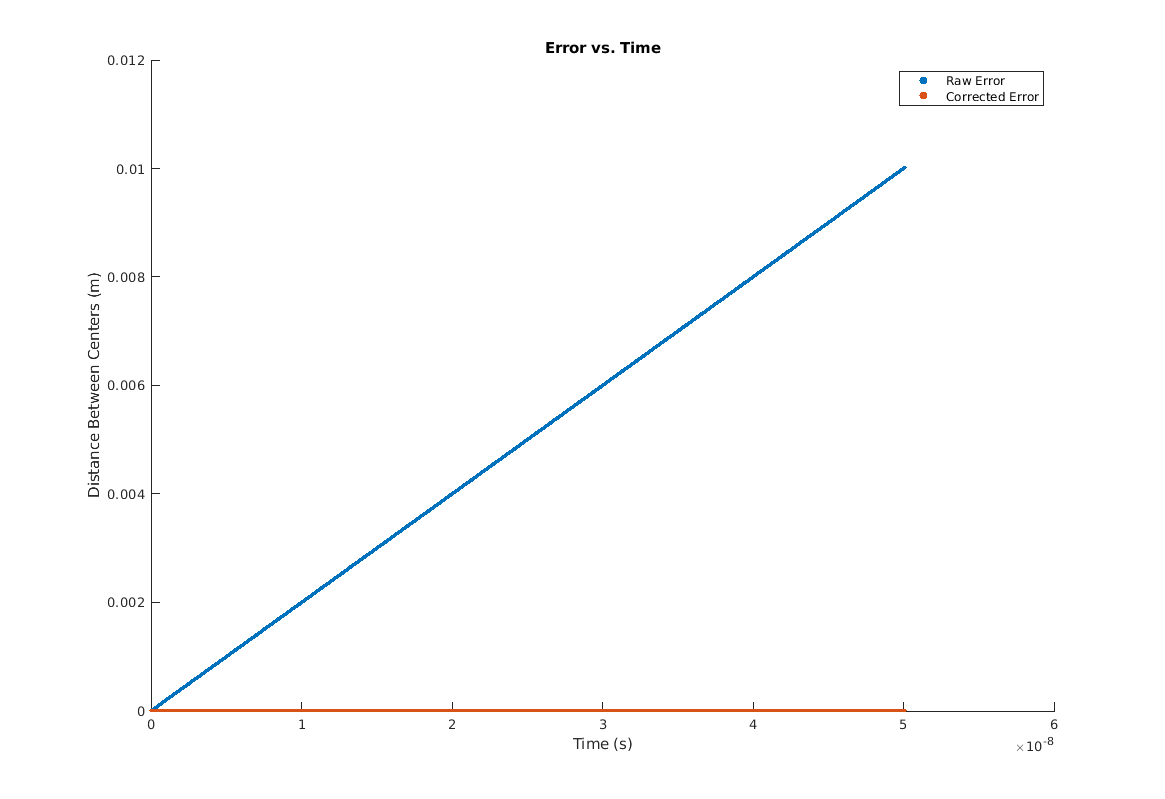
\includegraphics[width=0.7\linewidth]{drift2.png}
    \caption{Drift Over Time}
    \end{figure}

We also observe that the clustering of errors creates a clearly defined linear slope as time increases. This is indicative of a constant velocity drift from the expected center. We also find that when compared to the error trend of the corrected simulation the drift is nearly zero. 

\section{Trapping Field}

Next, we advance the simulation by establishing a solenoidal B-field in the opposite direction of the global $1~$T B-Field around the geometry. The solenoidal field is placed such that it reduces the net magnetic field at the center of the trap to $0.9~$T. 

    \begin{figure}[H]
    \centering
    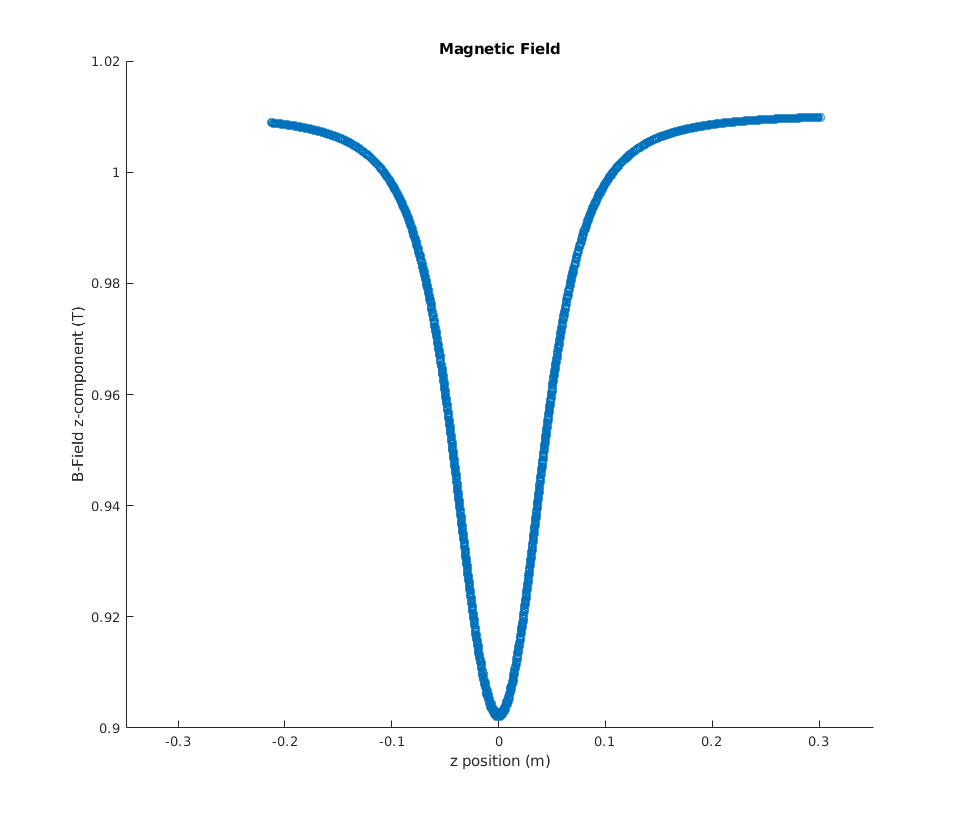
\includegraphics[width=0.7\linewidth]{solenoid.png}
    \caption{Visualization of B-Field Experienced by Particles in Trap}
    \end{figure}

This creates a trapping field that should contain electrons below a certain z momentum.

\subsection{Oscillation Behavior}

We expect to see a critical pitch angle (angle of the initial momentum to the positive z-axis) at which the z momentum is low enough for electrons to be trapped. Using the existing particle generator at the center of the geometry with an isotropic distribution we can visualize that critical angle and also examine the characteristics of the magnetron motion of the electron. 

    \begin{figure}[H]
    \centering
    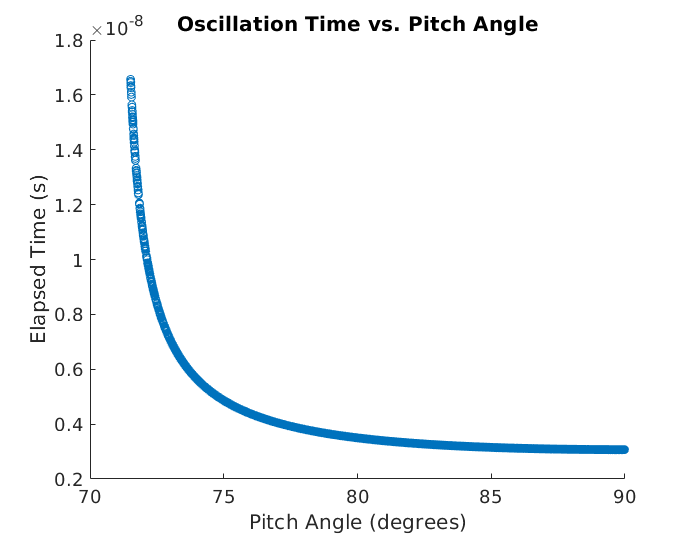
\includegraphics[width=0.7\linewidth]{oscillationtime.png}
    \caption{Time of flight of trapped electrons between the classical turning points}
    \end{figure}
    
    \begin{figure}[H]
    \centering
    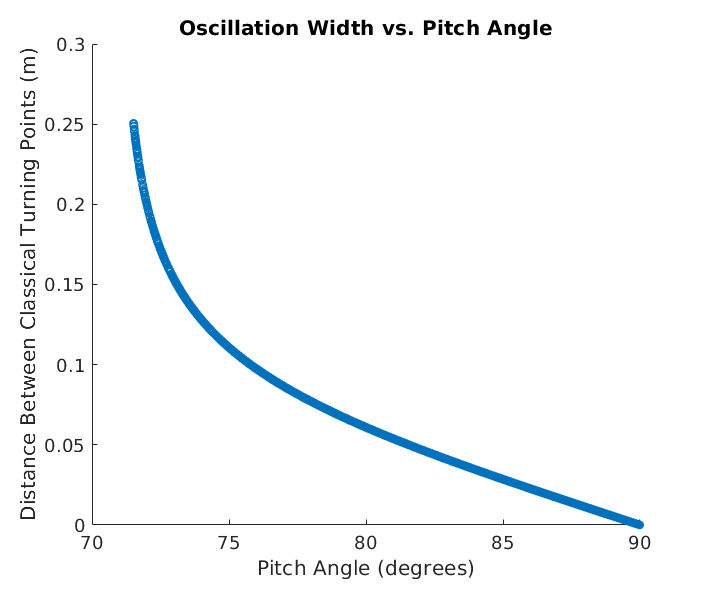
\includegraphics[width=0.7\linewidth]{oscillationwidth.png}
    \caption{Width of magnetron motion}
    \end{figure}

The two figures above characterize the magnetron motion of the electrons as it relates to the pitch angle of the electron. We observe that the critical angle is around $72~$degrees where any trapped electron has a greater pitch angle than that. 

We also observe that the oscillation time rapidly decreases with pitch angle to an asymtope of around $2~$ns. The constant time from angles greater than $80~$degrees suggests that the magnetic field is parabolic in this range.

We observe that the oscillation width of the magnetron motion decreases to zero as it approaches $90~$degrees as expected. Between these two profiles of the electron motion and the profile of the magnetic field, we conclude that the simulation is behaving as intended. 

\subsection{Trapping Fraction}

To characterize this trap we calculate the trapping fraction, the ratio between the trapped particles and the total number of particles generated. We define a trapped particle as a particle that has existed for more than 10000 simulation steps without encountering a trap boundary (radius of $1~$cm and z position of $\pm30~$cm).

For the isotropic distribution of electrons generated at the center of the trap with a kinetic energy of $511~$keV the trapping fraction is $33.6$\% (N = 1000).

The simulation was also altered to generate particles uniformly within the trapping geometry rather than just at the center. It was also modified such that the particle could be generated with a momentum vector pointed in any direction from the particle while maintaining an isotropic distribution of velocity along the z-axis. This represents a more accurate approach to what would be seen in the CRES experiment. The trapping fraction under these condition is $8.341$\% (N = 100000). 

It is worth noting that for the first trapping fraction, a particle either escaped out of the trap in the z direction due to high momentum or was trapped. For the trapping fraction for the uniform particle placement there were a number of scenarios where the larmor radius exceeded the trap geometry and encountered the maximum radius of the geometry. These particles accounted for $21.3$\% of particles and were never granted the opportunity to be trapped and generally survived for less than 10 steps of the simulation. 

\section{Trap with E-Field Sweep}
Finally, we alter the trap geometry defined in the previous section to include the same E-field defined in section 3. This is an E-field in the negative y direction with a magnitude of $2\times10^5~$V/m. 

Using this geometry, we analyze the time it takes trapped electrons to evacuate the trap. We do this by generating particles using the uniform distribution described in the previous section and examining their behavior.

First, we filter particles that were not trapped by eliminating particles that had a lifetime of less than 1000 steps, this eliminates particles described in the previous section whose larmor radius was too large to be contained in the trap initially. We also filter more particles that were not trapped by eliminating particles that exceeded the z-axis limits of the trap. This eliminates particles that either had a too great z momentum to be trapped or that were generated too close to the boundary of the trap to be trapped by the B-field.

Taking the particles that remained from the filter method described above, and plotting the time between the generation of these particles and when they encountered the boundary of the geometry yields a histogram of trap emptying times for the population of trapped electrons. 

    \begin{figure}[H]
    \centering
    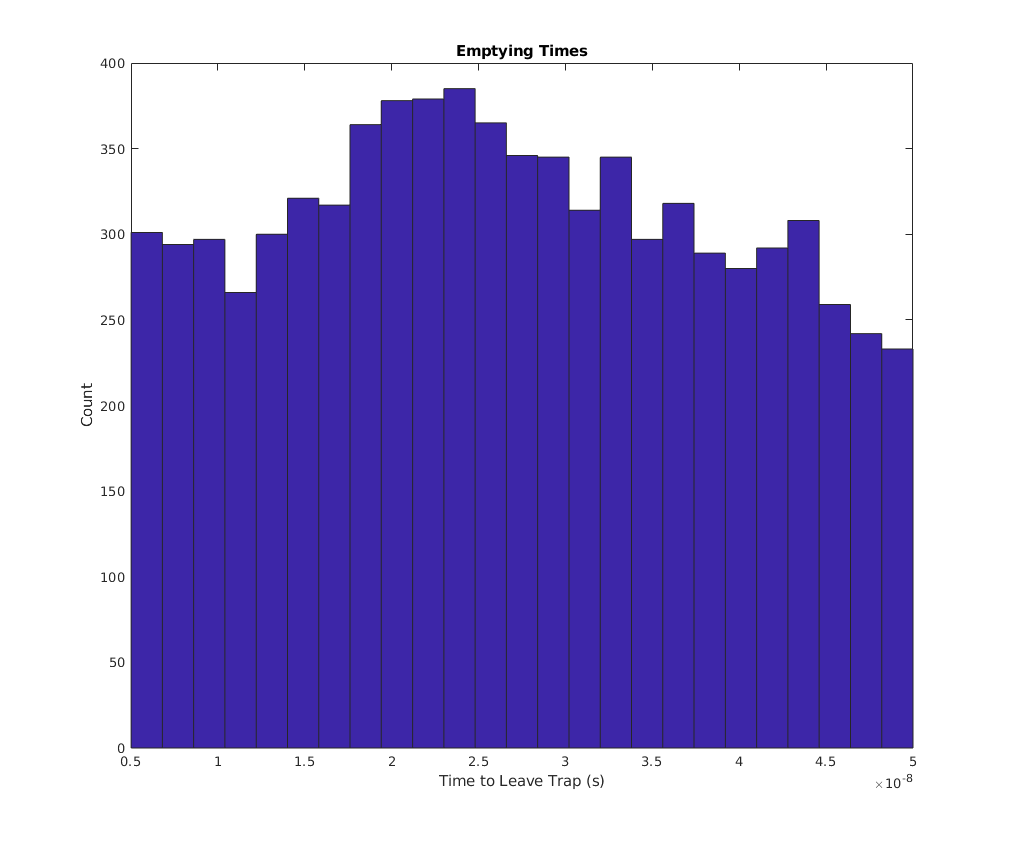
\includegraphics[width=0.7\linewidth]{emptying.png}
    \caption{Histogram of Emptying Times (N = 7835)}
    \end{figure}

Here we see that the escape times of the electrons are confined within $5~$ns to $50~$ns bounds with a relatively uniform distribution other than a shallow peak at around $20~$ns. This is a good first estimate of the emptying time of the real experiment, and due to the orders of magnitude present we conclude that the proposed electric field will be more than necessary to empty the trap in a reasonable period of time and that the field could likely be reduced as well. 

\section{Appendix}

Code used to generate the figures in this document is accessible \href{https://github.ncsu.edu/arallen4/CRES/blob/master/ConstantField.xml}{here}. The data used to generate these figures is on the server the simulations were run on. Please contact Alexander Allen (arallen4@ncsu.edu) for access. 


\end{document}

